\documentclass[twoside]{book}

% Packages required by doxygen
\usepackage{fixltx2e}
\usepackage{calc}
\usepackage{doxygen}
\usepackage[export]{adjustbox} % also loads graphicx
\usepackage{graphicx}
\usepackage[utf8]{inputenc}
\usepackage{makeidx}
\usepackage{multicol}
\usepackage{multirow}
\PassOptionsToPackage{warn}{textcomp}
\usepackage{textcomp}
\usepackage[nointegrals]{wasysym}
\usepackage[table]{xcolor}

% Font selection
\usepackage[T1]{fontenc}
\usepackage[scaled=.90]{helvet}
\usepackage{courier}
\usepackage{amssymb}
\usepackage{sectsty}
\renewcommand{\familydefault}{\sfdefault}
\allsectionsfont{%
  \fontseries{bc}\selectfont%
  \color{darkgray}%
}
\renewcommand{\DoxyLabelFont}{%
  \fontseries{bc}\selectfont%
  \color{darkgray}%
}
\newcommand{\+}{\discretionary{\mbox{\scriptsize$\hookleftarrow$}}{}{}}

% Page & text layout
\usepackage{geometry}
\geometry{%
  a4paper,%
  top=2.5cm,%
  bottom=2.5cm,%
  left=2.5cm,%
  right=2.5cm%
}
\tolerance=750
\hfuzz=15pt
\hbadness=750
\setlength{\emergencystretch}{15pt}
\setlength{\parindent}{0cm}
\setlength{\parskip}{0.2cm}
\makeatletter
\renewcommand{\paragraph}{%
  \@startsection{paragraph}{4}{0ex}{-1.0ex}{1.0ex}{%
    \normalfont\normalsize\bfseries\SS@parafont%
  }%
}
\renewcommand{\subparagraph}{%
  \@startsection{subparagraph}{5}{0ex}{-1.0ex}{1.0ex}{%
    \normalfont\normalsize\bfseries\SS@subparafont%
  }%
}
\makeatother

% Headers & footers
\usepackage{fancyhdr}
\pagestyle{fancyplain}
\fancyhead[LE]{\fancyplain{}{\bfseries\thepage}}
\fancyhead[CE]{\fancyplain{}{}}
\fancyhead[RE]{\fancyplain{}{\bfseries\leftmark}}
\fancyhead[LO]{\fancyplain{}{\bfseries\rightmark}}
\fancyhead[CO]{\fancyplain{}{}}
\fancyhead[RO]{\fancyplain{}{\bfseries\thepage}}
\fancyfoot[LE]{\fancyplain{}{}}
\fancyfoot[CE]{\fancyplain{}{}}
\fancyfoot[RE]{\fancyplain{}{\bfseries\scriptsize Generated on Wed Mar 18 2015 02\+:25\+:49 for My Project by Doxygen }}
\fancyfoot[LO]{\fancyplain{}{\bfseries\scriptsize Generated on Wed Mar 18 2015 02\+:25\+:49 for My Project by Doxygen }}
\fancyfoot[CO]{\fancyplain{}{}}
\fancyfoot[RO]{\fancyplain{}{}}
\renewcommand{\footrulewidth}{0.4pt}
\renewcommand{\chaptermark}[1]{%
  \markboth{#1}{}%
}
\renewcommand{\sectionmark}[1]{%
  \markright{\thesection\ #1}%
}

% Indices & bibliography
\usepackage{natbib}
\usepackage[titles]{tocloft}
\setcounter{tocdepth}{3}
\setcounter{secnumdepth}{5}
\makeindex

% Hyperlinks (required, but should be loaded last)
\usepackage{ifpdf}
\ifpdf
  \usepackage[pdftex,pagebackref=true]{hyperref}
\else
  \usepackage[ps2pdf,pagebackref=true]{hyperref}
\fi
\hypersetup{%
  colorlinks=true,%
  linkcolor=blue,%
  citecolor=blue,%
  unicode%
}

% Custom commands
\newcommand{\clearemptydoublepage}{%
  \newpage{\pagestyle{empty}\cleardoublepage}%
}


%===== C O N T E N T S =====

\begin{document}

% Titlepage & ToC
\hypersetup{pageanchor=false,
             bookmarks=true,
             bookmarksnumbered=true,
             pdfencoding=unicode
            }
\pagenumbering{roman}
\begin{titlepage}
\vspace*{7cm}
\begin{center}%
{\Large My Project }\\
\vspace*{1cm}
{\large Generated by Doxygen 1.8.9.1}\\
\vspace*{0.5cm}
{\small Wed Mar 18 2015 02:25:49}\\
\end{center}
\end{titlepage}
\clearemptydoublepage
\tableofcontents
\clearemptydoublepage
\pagenumbering{arabic}
\hypersetup{pageanchor=true}

%--- Begin generated contents ---
\chapter{Hierarchical Index}
\section{Class Hierarchy}
This inheritance list is sorted roughly, but not completely, alphabetically\+:\begin{DoxyCompactList}
\item \contentsline{section}{Arab\+Exp}{\pageref{class_arab_exp}}{}
\item \contentsline{section}{Bilangan}{\pageref{class_bilangan}}{}
\begin{DoxyCompactList}
\item \contentsline{section}{Arab}{\pageref{class_arab}}{}
\item \contentsline{section}{Romawi}{\pageref{class_romawi}}{}
\end{DoxyCompactList}
\item \contentsline{section}{Ekspresi}{\pageref{class_ekspresi}}{}
\begin{DoxyCompactList}
\item \contentsline{section}{Aritmatik}{\pageref{class_aritmatik}}{}
\begin{DoxyCompactList}
\item \contentsline{section}{Arab}{\pageref{class_arab}}{}
\item \contentsline{section}{Romawi}{\pageref{class_romawi}}{}
\end{DoxyCompactList}
\item \contentsline{section}{Boolean}{\pageref{class_boolean}}{}
\end{DoxyCompactList}
\item \contentsline{section}{Romawi\+Exp}{\pageref{class_romawi_exp}}{}
\end{DoxyCompactList}

\chapter{Class Index}
\section{Class List}
Here are the classes, structs, unions and interfaces with brief descriptions\+:\begin{DoxyCompactList}
\item\contentsline{section}{\hyperlink{class_history}{History} }{\pageref{class_history}}{}
\item\contentsline{section}{\hyperlink{classstack}{stack$<$ T $>$} }{\pageref{classstack}}{}
\end{DoxyCompactList}

\chapter{Class Documentation}
\hypertarget{class_arab}{}\section{Arab Class Reference}
\label{class_arab}\index{Arab@{Arab}}


{\ttfamily \#include $<$Arab.\+h$>$}

Inheritance diagram for Arab\+:\begin{figure}[H]
\begin{center}
\leavevmode
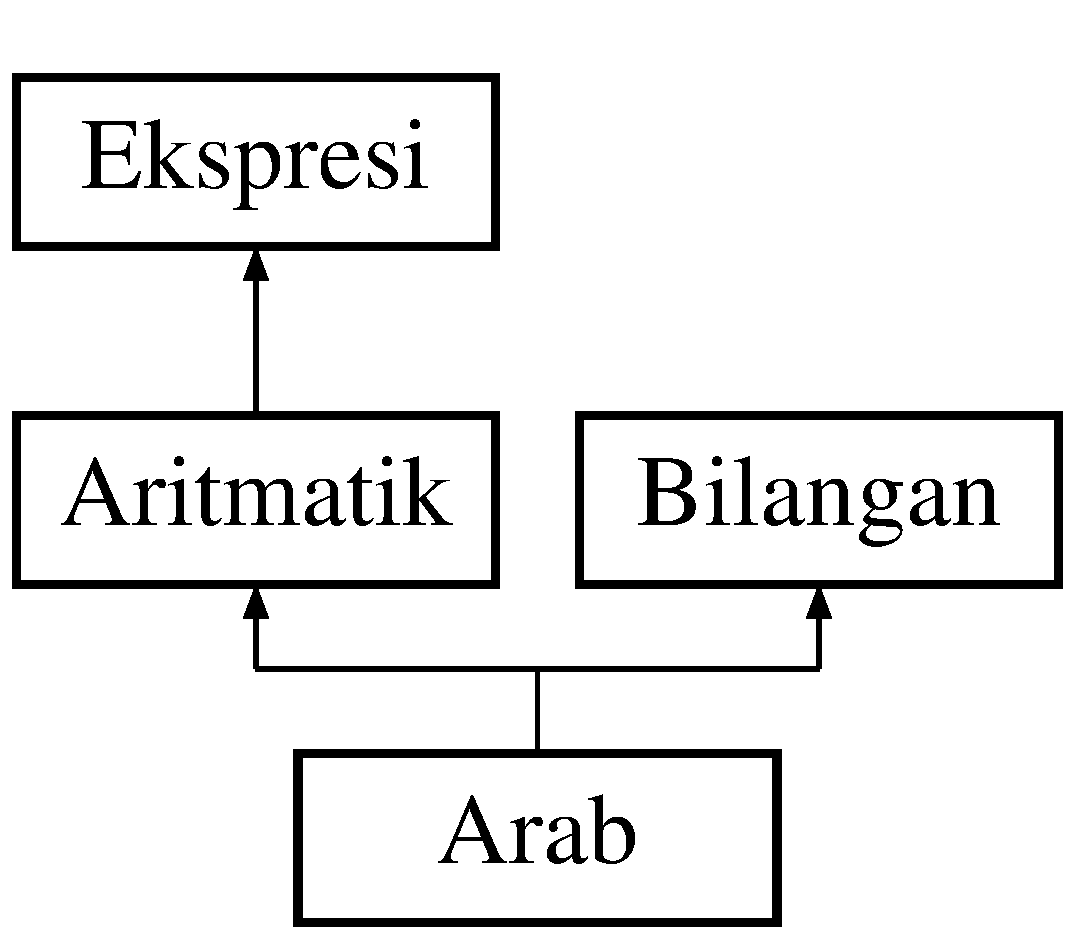
\includegraphics[height=3.000000cm]{class_arab}
\end{center}
\end{figure}
\subsection*{Public Member Functions}
\begin{DoxyCompactItemize}
\item 
\hyperlink{class_arab_afdddf6ff9c7724ddb71c625db0847893}{Arab} ()
\item 
\hyperlink{class_arab_a980e87ff4bcc914e8206b8850bc19f2b}{Arab} (std\+::string, int)
\item 
\hyperlink{class_arab_a2629b0540731753334ebb19161774f7a}{$\sim$\+Arab} ()
\item 
int \hyperlink{class_arab_a0200f0365cfc5ef5a35cac273f86ad0b}{calculate} ()
\item 
int \hyperlink{class_arab_aa9dfc0b92e76397bbd905ceeeebeaa45}{binary\+Opt} (std\+::string, int, int)
\item 
int \hyperlink{class_arab_a7dd22fd64705866419cc5b73c7231959}{unary\+Opt} (std\+::string, int)
\item 
int \hyperlink{class_arab_aa8eac0f26197eb68fa1753a7c33a6f2c}{to\+Int} (std\+::string)
\item 
std\+::string \hyperlink{class_arab_a051a742948dbc9f296b05436af050b4d}{to\+String} (int)
\end{DoxyCompactItemize}
\subsection*{Additional Inherited Members}


\subsection{Detailed Description}
\hyperlink{class_arab}{Arab} class. menangani ekspresi yang berupa bilangan arab, turunan dari kelas \hyperlink{class_aritmatik}{Aritmatik} dan Mengimplementasi interface dari \hyperlink{class_bilangan}{Bilangan}. 

\subsection{Constructor \& Destructor Documentation}
\hypertarget{class_arab_afdddf6ff9c7724ddb71c625db0847893}{}\index{Arab@{Arab}!Arab@{Arab}}
\index{Arab@{Arab}!Arab@{Arab}}
\subsubsection[{Arab}]{\setlength{\rightskip}{0pt plus 5cm}Arab\+::\+Arab (
\begin{DoxyParamCaption}
{}
\end{DoxyParamCaption}
)}\label{class_arab_afdddf6ff9c7724ddb71c625db0847893}
A constructor. Membuat Objek \hyperlink{class_aritmatik}{Aritmatik} \hypertarget{class_arab_a980e87ff4bcc914e8206b8850bc19f2b}{}\index{Arab@{Arab}!Arab@{Arab}}
\index{Arab@{Arab}!Arab@{Arab}}
\subsubsection[{Arab}]{\setlength{\rightskip}{0pt plus 5cm}Arab\+::\+Arab (
\begin{DoxyParamCaption}
\item[{std\+::string}]{eks, }
\item[{int}]{\+\_\+mode}
\end{DoxyParamCaption}
)}\label{class_arab_a980e87ff4bcc914e8206b8850bc19f2b}
A constructor. Membuat Objek \hyperlink{class_aritmatik}{Aritmatik} 
\begin{DoxyParams}{Parameters}
{\em eks} & sebuah string \\
\hline
{\em mode} & a yang berupa integer \\
\hline
\end{DoxyParams}
\hypertarget{class_arab_a2629b0540731753334ebb19161774f7a}{}\index{Arab@{Arab}!````~Arab@{$\sim$\+Arab}}
\index{````~Arab@{$\sim$\+Arab}!Arab@{Arab}}
\subsubsection[{$\sim$\+Arab}]{\setlength{\rightskip}{0pt plus 5cm}Arab\+::$\sim$\+Arab (
\begin{DoxyParamCaption}
{}
\end{DoxyParamCaption}
)}\label{class_arab_a2629b0540731753334ebb19161774f7a}
A destructor. 

\subsection{Member Function Documentation}
\hypertarget{class_arab_aa9dfc0b92e76397bbd905ceeeebeaa45}{}\index{Arab@{Arab}!binary\+Opt@{binary\+Opt}}
\index{binary\+Opt@{binary\+Opt}!Arab@{Arab}}
\subsubsection[{binary\+Opt}]{\setlength{\rightskip}{0pt plus 5cm}int Arab\+::binary\+Opt (
\begin{DoxyParamCaption}
\item[{std\+::string}]{oprt, }
\item[{int}]{a, }
\item[{int}]{b}
\end{DoxyParamCaption}
)\hspace{0.3cm}{\ttfamily [virtual]}}\label{class_arab_aa9dfc0b92e76397bbd905ceeeebeaa45}
Method yang mengembalikan hasil dari operasi binary Menghitung dua buah integer 
\begin{DoxyParams}{Parameters}
{\em a} & sebuah integer \\
\hline
{\em b} & sebuah integer \\
\hline
\end{DoxyParams}
\begin{DoxyReturn}{Returns}
hasil perhitungan binary 
\end{DoxyReturn}


Implements \hyperlink{class_bilangan_acb958e0fade6bdfc3b6ce88bf57560bc}{Bilangan}.

\hypertarget{class_arab_a0200f0365cfc5ef5a35cac273f86ad0b}{}\index{Arab@{Arab}!calculate@{calculate}}
\index{calculate@{calculate}!Arab@{Arab}}
\subsubsection[{calculate}]{\setlength{\rightskip}{0pt plus 5cm}int Arab\+::calculate (
\begin{DoxyParamCaption}
{}
\end{DoxyParamCaption}
)\hspace{0.3cm}{\ttfamily [virtual]}}\label{class_arab_a0200f0365cfc5ef5a35cac273f86ad0b}
Method yang mengembalikan hasil perhitungan Menghitung string postfix dengan stack. \begin{DoxySeeAlso}{See also}
\hyperlink{class_arab_aa9dfc0b92e76397bbd905ceeeebeaa45}{binary\+Opt} 

\hyperlink{class_arab_a7dd22fd64705866419cc5b73c7231959}{unary\+Opt} 

\hyperlink{class_arab_aa8eac0f26197eb68fa1753a7c33a6f2c}{to\+Int} 
\end{DoxySeeAlso}
\begin{DoxyReturn}{Returns}
hasil perhitungan 
\end{DoxyReturn}


Implements \hyperlink{class_bilangan_a519c33685bdc47e8386037ac8d2bfaa6}{Bilangan}.

\hypertarget{class_arab_aa8eac0f26197eb68fa1753a7c33a6f2c}{}\index{Arab@{Arab}!to\+Int@{to\+Int}}
\index{to\+Int@{to\+Int}!Arab@{Arab}}
\subsubsection[{to\+Int}]{\setlength{\rightskip}{0pt plus 5cm}int Arab\+::to\+Int (
\begin{DoxyParamCaption}
\item[{std\+::string}]{str}
\end{DoxyParamCaption}
)\hspace{0.3cm}{\ttfamily [virtual]}}\label{class_arab_aa8eac0f26197eb68fa1753a7c33a6f2c}
Method yang mengembalikan integet Mengubah string menjadi Integer 
\begin{DoxyParams}{Parameters}
{\em str} & sebuah string \\
\hline
\end{DoxyParams}
\begin{DoxyReturn}{Returns}
bilangan integer hasil convert 
\end{DoxyReturn}


Implements \hyperlink{class_bilangan_ab4fd66bd8e9179176f97f8b856eda103}{Bilangan}.

\hypertarget{class_arab_a051a742948dbc9f296b05436af050b4d}{}\index{Arab@{Arab}!to\+String@{to\+String}}
\index{to\+String@{to\+String}!Arab@{Arab}}
\subsubsection[{to\+String}]{\setlength{\rightskip}{0pt plus 5cm}std\+::string Arab\+::to\+String (
\begin{DoxyParamCaption}
\item[{int}]{bil}
\end{DoxyParamCaption}
)\hspace{0.3cm}{\ttfamily [virtual]}}\label{class_arab_a051a742948dbc9f296b05436af050b4d}
Method yang mengembalikan string Mengubah Integer menjadi string 
\begin{DoxyParams}{Parameters}
{\em bil} & sebuah integer \\
\hline
\end{DoxyParams}
\begin{DoxyReturn}{Returns}
the string 
\end{DoxyReturn}


Implements \hyperlink{class_bilangan_ac712d0d2b78dabad769b0b1e9cef8dc6}{Bilangan}.

\hypertarget{class_arab_a7dd22fd64705866419cc5b73c7231959}{}\index{Arab@{Arab}!unary\+Opt@{unary\+Opt}}
\index{unary\+Opt@{unary\+Opt}!Arab@{Arab}}
\subsubsection[{unary\+Opt}]{\setlength{\rightskip}{0pt plus 5cm}int Arab\+::unary\+Opt (
\begin{DoxyParamCaption}
\item[{std\+::string}]{oprt, }
\item[{int}]{a}
\end{DoxyParamCaption}
)\hspace{0.3cm}{\ttfamily [virtual]}}\label{class_arab_a7dd22fd64705866419cc5b73c7231959}
Method yang mengembalikan hasil dari operasi unary Menghitung satu buah integer 
\begin{DoxyParams}{Parameters}
{\em a} & sebuah integer \\
\hline
\end{DoxyParams}
\begin{DoxyReturn}{Returns}
bilangan integer sebuah hasil 
\end{DoxyReturn}


Implements \hyperlink{class_bilangan_af812d372ad4de1afe2e6a4dc9e8f95ef}{Bilangan}.



The documentation for this class was generated from the following files\+:\begin{DoxyCompactItemize}
\item 
Arab.\+h\item 
Arab.\+cpp\end{DoxyCompactItemize}

\hypertarget{class_arab_exp}{}\section{Arab\+Exp Class Reference}
\label{class_arab_exp}\index{Arab\+Exp@{Arab\+Exp}}


{\ttfamily \#include $<$Arab\+Exp.\+h$>$}

\subsection*{Public Member Functions}
\begin{DoxyCompactItemize}
\item 
\hyperlink{class_arab_exp_ab93ffaec3e5eba1c2f6f19484359ea30}{Arab\+Exp} (int)
\item 
\hyperlink{class_arab_exp_af5eb5d741a5450b9a1c1b04173d5105c}{Arab\+Exp} (const \hyperlink{class_arab_exp}{Arab\+Exp} \&)
\item 
void \hyperlink{class_arab_exp_a7374de037107c12d3231816ee7cb8b83}{display\+Msg} ()
\end{DoxyCompactItemize}


\subsection{Detailed Description}
\hyperlink{class_arab_exp}{Arab\+Exp} class. menangani input yang tidak memungkinkan output, seperti dibagi dengan nol 

\subsection{Constructor \& Destructor Documentation}
\hypertarget{class_arab_exp_ab93ffaec3e5eba1c2f6f19484359ea30}{}\index{Arab\+Exp@{Arab\+Exp}!Arab\+Exp@{Arab\+Exp}}
\index{Arab\+Exp@{Arab\+Exp}!Arab\+Exp@{Arab\+Exp}}
\subsubsection[{Arab\+Exp}]{\setlength{\rightskip}{0pt plus 5cm}Arab\+Exp\+::\+Arab\+Exp (
\begin{DoxyParamCaption}
\item[{int}]{id}
\end{DoxyParamCaption}
)}\label{class_arab_exp_ab93ffaec3e5eba1c2f6f19484359ea30}
A constructor. Memnginisialisasi msg\+\_\+id = id dengan ctor initilization list 
\begin{DoxyParams}{Parameters}
{\em id} & sebagai int \\
\hline
\end{DoxyParams}
\hypertarget{class_arab_exp_af5eb5d741a5450b9a1c1b04173d5105c}{}\index{Arab\+Exp@{Arab\+Exp}!Arab\+Exp@{Arab\+Exp}}
\index{Arab\+Exp@{Arab\+Exp}!Arab\+Exp@{Arab\+Exp}}
\subsubsection[{Arab\+Exp}]{\setlength{\rightskip}{0pt plus 5cm}Arab\+Exp\+::\+Arab\+Exp (
\begin{DoxyParamCaption}
\item[{const {\bf Arab\+Exp} \&}]{exp}
\end{DoxyParamCaption}
)}\label{class_arab_exp_af5eb5d741a5450b9a1c1b04173d5105c}
A copy constructor. Memnginisialisasi msg\+\_\+id = exp.\+msg\+\_\+id dengan ctor initilization list 
\begin{DoxyParams}{Parameters}
{\em exp} & sebagai konstanta reference dari \hyperlink{class_arab_exp}{Arab\+Exp} \\
\hline
\end{DoxyParams}


\subsection{Member Function Documentation}
\hypertarget{class_arab_exp_a7374de037107c12d3231816ee7cb8b83}{}\index{Arab\+Exp@{Arab\+Exp}!display\+Msg@{display\+Msg}}
\index{display\+Msg@{display\+Msg}!Arab\+Exp@{Arab\+Exp}}
\subsubsection[{display\+Msg}]{\setlength{\rightskip}{0pt plus 5cm}void Arab\+Exp\+::display\+Msg (
\begin{DoxyParamCaption}
{}
\end{DoxyParamCaption}
)}\label{class_arab_exp_a7374de037107c12d3231816ee7cb8b83}
A void to display the string ( msg\mbox{[}\mbox{]}). Memngoutput msg\mbox{[}msg\+\_\+id\mbox{]} 

The documentation for this class was generated from the following files\+:\begin{DoxyCompactItemize}
\item 
Arab\+Exp.\+h\item 
Arab\+Exp.\+cpp\end{DoxyCompactItemize}

\hypertarget{class_aritmatik}{}\section{Aritmatik Class Reference}
\label{class_aritmatik}\index{Aritmatik@{Aritmatik}}


{\ttfamily \#include $<$Aritmatik.\+h$>$}

Inheritance diagram for Aritmatik\+:\begin{figure}[H]
\begin{center}
\leavevmode
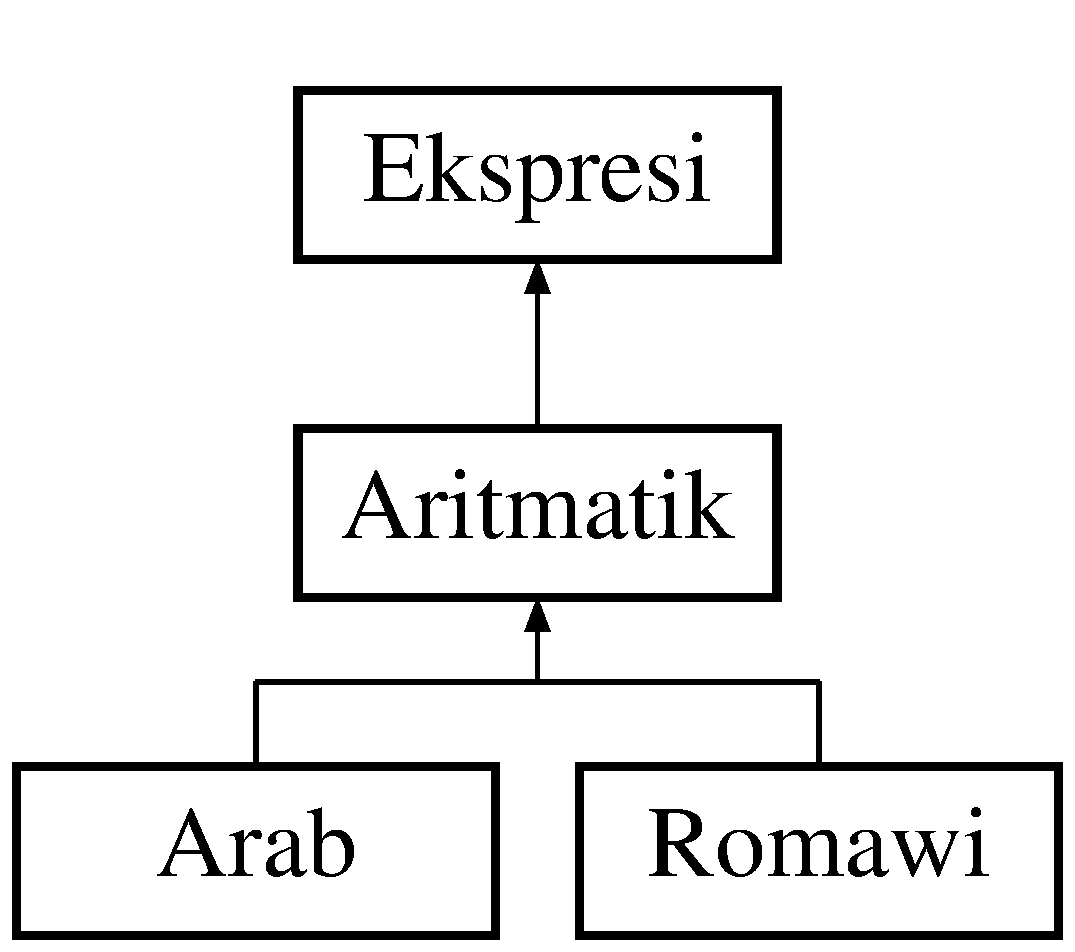
\includegraphics[height=3.000000cm]{class_aritmatik}
\end{center}
\end{figure}
\subsection*{Public Member Functions}
\begin{DoxyCompactItemize}
\item 
\hyperlink{class_aritmatik_aa7da5dc54ef0b249411dcd39def1cd39}{Aritmatik} ()
\item 
\hyperlink{class_aritmatik_ab399b33108b9a947b3ceb4b980c17949}{Aritmatik} (std\+::string, int)
\item 
\hyperlink{class_aritmatik_a418c3d95a5648adb083cacb09d63f0aa}{$\sim$\+Aritmatik} ()
\item 
bool \hyperlink{class_aritmatik_ad3bebd263fb4d94e850848c282f80d6b}{is\+Operan} (std\+::string)
\item 
bool \hyperlink{class_aritmatik_a22df02b3a845fd0af3e1bae28121ba99}{is\+Operator} (std\+::string)
\item 
bool \hyperlink{class_aritmatik_a2bdb89adcf3b187382a40f3c66e8b649}{higher\+Precedence} (std\+::string, std\+::string)
\end{DoxyCompactItemize}
\subsection*{Protected Member Functions}
\begin{DoxyCompactItemize}
\item 
int \hyperlink{class_aritmatik_acb650d44adc6254fb3e0f027838af2db}{get\+Operator\+Weight} (std\+::string)
\end{DoxyCompactItemize}
\subsection*{Additional Inherited Members}


\subsection{Detailed Description}
\hyperlink{class_aritmatik}{Aritmatik} class. menangani ekspresi yang menggunakan operator aritmatik, turunan dari kelas \hyperlink{class_ekspresi}{Ekspresi}. 

\subsection{Constructor \& Destructor Documentation}
\hypertarget{class_aritmatik_aa7da5dc54ef0b249411dcd39def1cd39}{}\index{Aritmatik@{Aritmatik}!Aritmatik@{Aritmatik}}
\index{Aritmatik@{Aritmatik}!Aritmatik@{Aritmatik}}
\subsubsection[{Aritmatik}]{\setlength{\rightskip}{0pt plus 5cm}Aritmatik\+::\+Aritmatik (
\begin{DoxyParamCaption}
{}
\end{DoxyParamCaption}
)}\label{class_aritmatik_aa7da5dc54ef0b249411dcd39def1cd39}
A constructor. Membuat Objek \hyperlink{class_ekspresi}{Ekspresi} \hypertarget{class_aritmatik_ab399b33108b9a947b3ceb4b980c17949}{}\index{Aritmatik@{Aritmatik}!Aritmatik@{Aritmatik}}
\index{Aritmatik@{Aritmatik}!Aritmatik@{Aritmatik}}
\subsubsection[{Aritmatik}]{\setlength{\rightskip}{0pt plus 5cm}Aritmatik\+::\+Aritmatik (
\begin{DoxyParamCaption}
\item[{std\+::string}]{eks, }
\item[{int}]{\+\_\+mode}
\end{DoxyParamCaption}
)}\label{class_aritmatik_ab399b33108b9a947b3ceb4b980c17949}
A constructor. Membuat Objek \hyperlink{class_aritmatik}{Aritmatik} dengan ekspresi 
\begin{DoxyParams}{Parameters}
{\em eks} & sebuah string \\
\hline
{\em mode} & yang berupa integer \\
\hline
\end{DoxyParams}
\hypertarget{class_aritmatik_a418c3d95a5648adb083cacb09d63f0aa}{}\index{Aritmatik@{Aritmatik}!````~Aritmatik@{$\sim$\+Aritmatik}}
\index{````~Aritmatik@{$\sim$\+Aritmatik}!Aritmatik@{Aritmatik}}
\subsubsection[{$\sim$\+Aritmatik}]{\setlength{\rightskip}{0pt plus 5cm}Aritmatik\+::$\sim$\+Aritmatik (
\begin{DoxyParamCaption}
{}
\end{DoxyParamCaption}
)}\label{class_aritmatik_a418c3d95a5648adb083cacb09d63f0aa}
A destructor. 

\subsection{Member Function Documentation}
\hypertarget{class_aritmatik_acb650d44adc6254fb3e0f027838af2db}{}\index{Aritmatik@{Aritmatik}!get\+Operator\+Weight@{get\+Operator\+Weight}}
\index{get\+Operator\+Weight@{get\+Operator\+Weight}!Aritmatik@{Aritmatik}}
\subsubsection[{get\+Operator\+Weight}]{\setlength{\rightskip}{0pt plus 5cm}int Aritmatik\+::get\+Operator\+Weight (
\begin{DoxyParamCaption}
\item[{std\+::string}]{oprt}
\end{DoxyParamCaption}
)\hspace{0.3cm}{\ttfamily [protected]}, {\ttfamily [virtual]}}\label{class_aritmatik_acb650d44adc6254fb3e0f027838af2db}
fungsi protected yang menghasilkan berat operator 
\begin{DoxyParams}{Parameters}
{\em oprt} & yang berupa string \\
\hline
\end{DoxyParams}
\begin{DoxyReturn}{Returns}
integer yang berupa bobot 
\end{DoxyReturn}


Implements \hyperlink{class_ekspresi_a1177f9babe3330a4f04adbac396e0e0e}{Ekspresi}.

\hypertarget{class_aritmatik_a2bdb89adcf3b187382a40f3c66e8b649}{}\index{Aritmatik@{Aritmatik}!higher\+Precedence@{higher\+Precedence}}
\index{higher\+Precedence@{higher\+Precedence}!Aritmatik@{Aritmatik}}
\subsubsection[{higher\+Precedence}]{\setlength{\rightskip}{0pt plus 5cm}bool Aritmatik\+::higher\+Precedence (
\begin{DoxyParamCaption}
\item[{std\+::string}]{high, }
\item[{std\+::string}]{low}
\end{DoxyParamCaption}
)\hspace{0.3cm}{\ttfamily [virtual]}}\label{class_aritmatik_a2bdb89adcf3b187382a40f3c66e8b649}
fungsi yang mengecek apakah string high mempunyai prioritas lebih tinggi dari string low 
\begin{DoxyParams}{Parameters}
{\em high} & yang berupa string \\
\hline
{\em low} & yang berupa string \\
\hline
\end{DoxyParams}
\begin{DoxyReturn}{Returns}
bool yang bernilai true jika string high $>$ string low 
\end{DoxyReturn}


Implements \hyperlink{class_ekspresi_a52ccbd282ee50c4c3d58eab0d662f0f9}{Ekspresi}.

\hypertarget{class_aritmatik_ad3bebd263fb4d94e850848c282f80d6b}{}\index{Aritmatik@{Aritmatik}!is\+Operan@{is\+Operan}}
\index{is\+Operan@{is\+Operan}!Aritmatik@{Aritmatik}}
\subsubsection[{is\+Operan}]{\setlength{\rightskip}{0pt plus 5cm}bool Aritmatik\+::is\+Operan (
\begin{DoxyParamCaption}
\item[{std\+::string}]{opr}
\end{DoxyParamCaption}
)\hspace{0.3cm}{\ttfamily [virtual]}}\label{class_aritmatik_ad3bebd263fb4d94e850848c282f80d6b}
fungsi yang mengecek apakah string berupa operan 
\begin{DoxyParams}{Parameters}
{\em opr} & yang berupa operan \\
\hline
\end{DoxyParams}
\begin{DoxyReturn}{Returns}
bool yang bernilai true jika string == operan 
\end{DoxyReturn}


Implements \hyperlink{class_ekspresi_ab742ee9ef7a7bc49ea9d3d96eae69e04}{Ekspresi}.

\hypertarget{class_aritmatik_a22df02b3a845fd0af3e1bae28121ba99}{}\index{Aritmatik@{Aritmatik}!is\+Operator@{is\+Operator}}
\index{is\+Operator@{is\+Operator}!Aritmatik@{Aritmatik}}
\subsubsection[{is\+Operator}]{\setlength{\rightskip}{0pt plus 5cm}bool Aritmatik\+::is\+Operator (
\begin{DoxyParamCaption}
\item[{std\+::string}]{oprt}
\end{DoxyParamCaption}
)\hspace{0.3cm}{\ttfamily [virtual]}}\label{class_aritmatik_a22df02b3a845fd0af3e1bae28121ba99}
fungsi yang mengecek apakah string berupa operator 
\begin{DoxyParams}{Parameters}
{\em opr} & yang berupa operator \\
\hline
\end{DoxyParams}
\begin{DoxyReturn}{Returns}
bool yang bernilai true jika string == operator 
\end{DoxyReturn}


Implements \hyperlink{class_ekspresi_a224d9cae2ee4d104d7ece7b853746dfc}{Ekspresi}.



The documentation for this class was generated from the following files\+:\begin{DoxyCompactItemize}
\item 
Aritmatik.\+h\item 
Aritmatik.\+cpp\end{DoxyCompactItemize}

\hypertarget{class_bilangan}{}\section{Bilangan Class Reference}
\label{class_bilangan}\index{Bilangan@{Bilangan}}
Inheritance diagram for Bilangan\+:\begin{figure}[H]
\begin{center}
\leavevmode
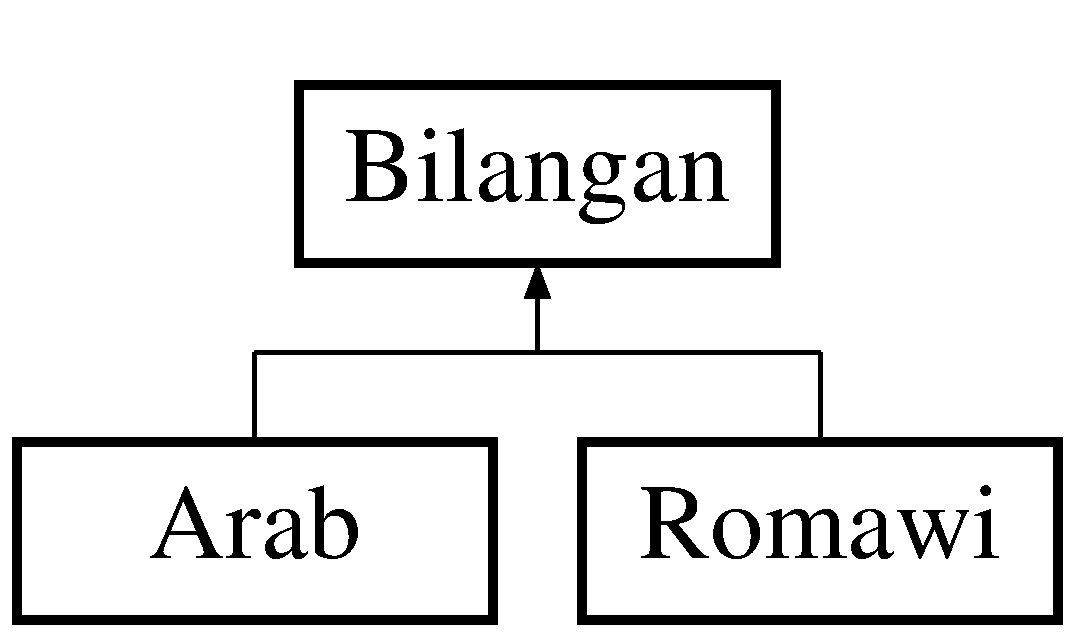
\includegraphics[height=2.000000cm]{class_bilangan}
\end{center}
\end{figure}
\subsection*{Public Member Functions}
\begin{DoxyCompactItemize}
\item 
virtual int \hyperlink{class_bilangan_a519c33685bdc47e8386037ac8d2bfaa6}{calculate} ()=0
\item 
virtual int \hyperlink{class_bilangan_acb958e0fade6bdfc3b6ce88bf57560bc}{binary\+Opt} (std\+::string, int, int)=0
\item 
virtual int \hyperlink{class_bilangan_af812d372ad4de1afe2e6a4dc9e8f95ef}{unary\+Opt} (std\+::string, int)=0
\item 
virtual int \hyperlink{class_bilangan_ab4fd66bd8e9179176f97f8b856eda103}{to\+Int} (std\+::string)=0
\item 
virtual std\+::string \hyperlink{class_bilangan_ac712d0d2b78dabad769b0b1e9cef8dc6}{to\+String} (int)=0
\end{DoxyCompactItemize}


\subsection{Member Function Documentation}
\hypertarget{class_bilangan_acb958e0fade6bdfc3b6ce88bf57560bc}{}\index{Bilangan@{Bilangan}!binary\+Opt@{binary\+Opt}}
\index{binary\+Opt@{binary\+Opt}!Bilangan@{Bilangan}}
\subsubsection[{binary\+Opt}]{\setlength{\rightskip}{0pt plus 5cm}virtual int Bilangan\+::binary\+Opt (
\begin{DoxyParamCaption}
\item[{std\+::string}]{, }
\item[{int}]{, }
\item[{int}]{}
\end{DoxyParamCaption}
)\hspace{0.3cm}{\ttfamily [pure virtual]}}\label{class_bilangan_acb958e0fade6bdfc3b6ce88bf57560bc}
A pure virtual member 
\begin{DoxyParams}{Parameters}
{\em a1} & angka1. \\
\hline
{\em a2} & angka2. \\
\hline
{\em str} & stringnya. \\
\hline
\end{DoxyParams}
\begin{DoxyReturn}{Returns}
hasil kalkulasi operasi biner 
\end{DoxyReturn}


Implemented in \hyperlink{class_arab_aa9dfc0b92e76397bbd905ceeeebeaa45}{Arab}, and \hyperlink{class_romawi_aaa81d7f110f3baabad7571fec567bb12}{Romawi}.

\hypertarget{class_bilangan_a519c33685bdc47e8386037ac8d2bfaa6}{}\index{Bilangan@{Bilangan}!calculate@{calculate}}
\index{calculate@{calculate}!Bilangan@{Bilangan}}
\subsubsection[{calculate}]{\setlength{\rightskip}{0pt plus 5cm}virtual int Bilangan\+::calculate (
\begin{DoxyParamCaption}
{}
\end{DoxyParamCaption}
)\hspace{0.3cm}{\ttfamily [pure virtual]}}\label{class_bilangan_a519c33685bdc47e8386037ac8d2bfaa6}
A pure virtual member. \begin{DoxyReturn}{Returns}
hasil kalkulasi seluruh string 
\end{DoxyReturn}


Implemented in \hyperlink{class_arab_a0200f0365cfc5ef5a35cac273f86ad0b}{Arab}, and \hyperlink{class_romawi_a6fabccebadf8807fbdd50a0c45b093e2}{Romawi}.

\hypertarget{class_bilangan_ab4fd66bd8e9179176f97f8b856eda103}{}\index{Bilangan@{Bilangan}!to\+Int@{to\+Int}}
\index{to\+Int@{to\+Int}!Bilangan@{Bilangan}}
\subsubsection[{to\+Int}]{\setlength{\rightskip}{0pt plus 5cm}virtual int Bilangan\+::to\+Int (
\begin{DoxyParamCaption}
\item[{std\+::string}]{}
\end{DoxyParamCaption}
)\hspace{0.3cm}{\ttfamily [pure virtual]}}\label{class_bilangan_ab4fd66bd8e9179176f97f8b856eda103}
A pure virtual member. 
\begin{DoxyParams}{Parameters}
{\em str} & stringnya. \\
\hline
\end{DoxyParams}
\begin{DoxyReturn}{Returns}
hasil konversi dari string ke integer 
\end{DoxyReturn}


Implemented in \hyperlink{class_arab_aa8eac0f26197eb68fa1753a7c33a6f2c}{Arab}, and \hyperlink{class_romawi_ae884d8a5a65c397fe53a05af8f0747f4}{Romawi}.

\hypertarget{class_bilangan_ac712d0d2b78dabad769b0b1e9cef8dc6}{}\index{Bilangan@{Bilangan}!to\+String@{to\+String}}
\index{to\+String@{to\+String}!Bilangan@{Bilangan}}
\subsubsection[{to\+String}]{\setlength{\rightskip}{0pt plus 5cm}virtual std\+::string Bilangan\+::to\+String (
\begin{DoxyParamCaption}
\item[{int}]{}
\end{DoxyParamCaption}
)\hspace{0.3cm}{\ttfamily [pure virtual]}}\label{class_bilangan_ac712d0d2b78dabad769b0b1e9cef8dc6}
A pure virtual member. 
\begin{DoxyParams}{Parameters}
{\em a} & angka1. \\
\hline
\end{DoxyParams}
\begin{DoxyReturn}{Returns}
hasil konversi dari int ke string 
\end{DoxyReturn}


Implemented in \hyperlink{class_arab_a051a742948dbc9f296b05436af050b4d}{Arab}, and \hyperlink{class_romawi_a338773fe7e1762d5c52e803ba2957205}{Romawi}.

\hypertarget{class_bilangan_af812d372ad4de1afe2e6a4dc9e8f95ef}{}\index{Bilangan@{Bilangan}!unary\+Opt@{unary\+Opt}}
\index{unary\+Opt@{unary\+Opt}!Bilangan@{Bilangan}}
\subsubsection[{unary\+Opt}]{\setlength{\rightskip}{0pt plus 5cm}virtual int Bilangan\+::unary\+Opt (
\begin{DoxyParamCaption}
\item[{std\+::string}]{, }
\item[{int}]{}
\end{DoxyParamCaption}
)\hspace{0.3cm}{\ttfamily [pure virtual]}}\label{class_bilangan_af812d372ad4de1afe2e6a4dc9e8f95ef}
A pure virtual member 
\begin{DoxyParams}{Parameters}
{\em a1} & angka1. \\
\hline
{\em str} & stringnya. \\
\hline
\end{DoxyParams}
\begin{DoxyReturn}{Returns}
hasil kalkulasi operasi unary 
\end{DoxyReturn}


Implemented in \hyperlink{class_arab_a7dd22fd64705866419cc5b73c7231959}{Arab}, and \hyperlink{class_romawi_af98f44a64aa48746641faac4dac3fb33}{Romawi}.



The documentation for this class was generated from the following file\+:\begin{DoxyCompactItemize}
\item 
Bilangan.\+h\end{DoxyCompactItemize}

\hypertarget{class_boolean}{}\section{Boolean Class Reference}
\label{class_boolean}\index{Boolean@{Boolean}}
Inheritance diagram for Boolean\+:\begin{figure}[H]
\begin{center}
\leavevmode
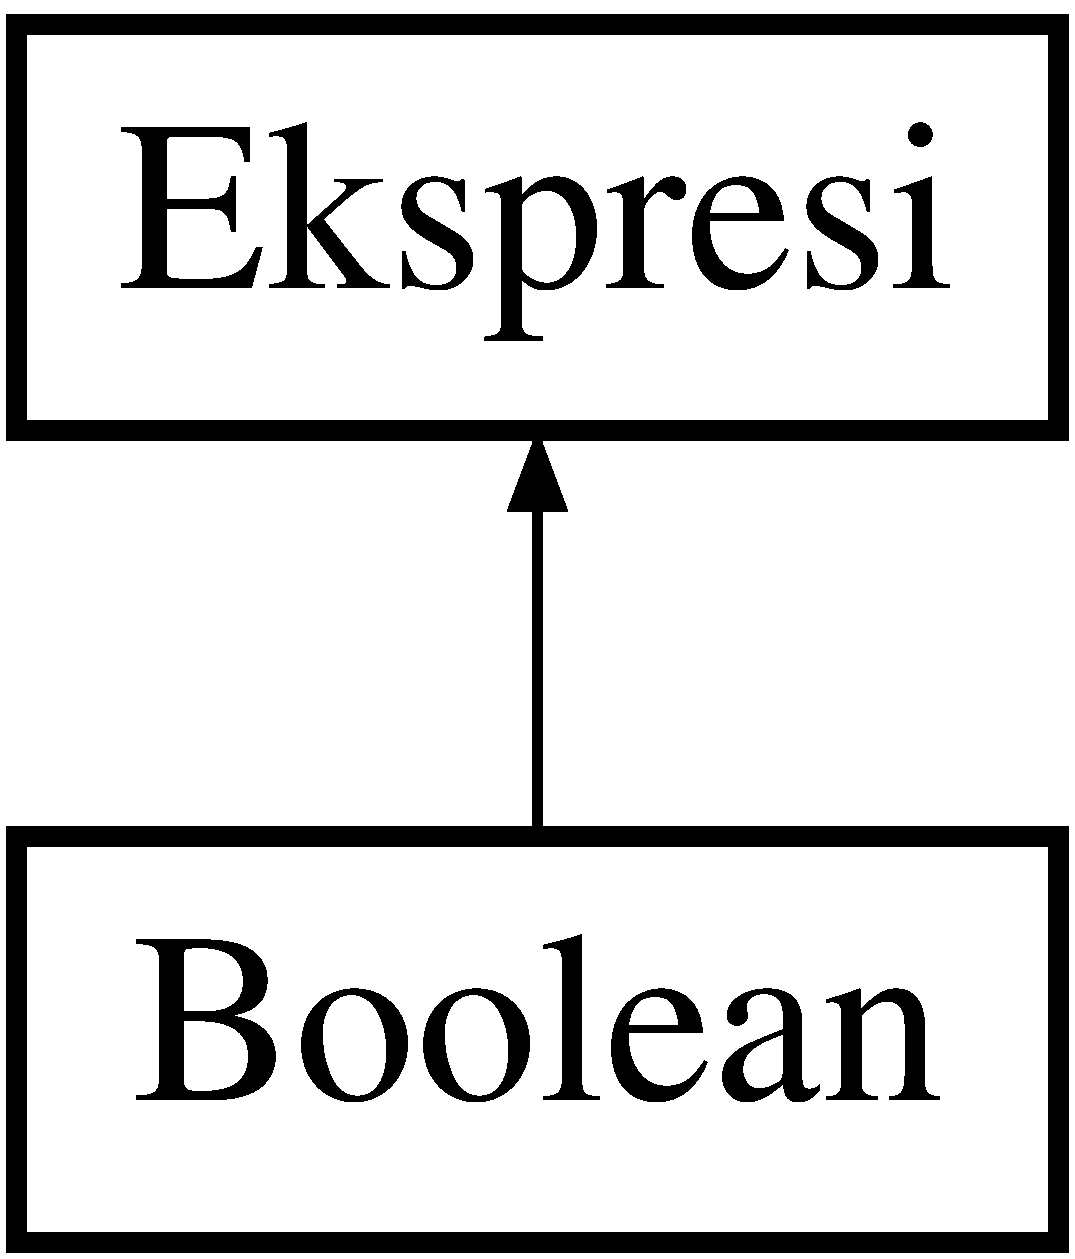
\includegraphics[height=2.000000cm]{class_boolean}
\end{center}
\end{figure}
\subsection*{Public Member Functions}
\begin{DoxyCompactItemize}
\item 
\hyperlink{class_boolean_a9acbc8d83926e3900765a64a34381244}{Boolean} ()
\item 
\hyperlink{class_boolean_ae880e02386228f33f2a737cda4454961}{Boolean} (std\+::string, int)
\item 
\hyperlink{class_boolean_a025bfd19cd093dbbe9492fdab16c056b}{$\sim$\+Boolean} ()
\item 
bool \hyperlink{class_boolean_a9c5afca5ecb28f04ac727a56d646d057}{is\+Operan} (std\+::string)
\item 
bool \hyperlink{class_boolean_a37e98802c20820e8cdbbfa38232b4930}{is\+Operator} (std\+::string)
\item 
bool \hyperlink{class_boolean_a98d763cbf5a4593f5ec268bf7ccd3553}{higher\+Precedence} (std\+::string, std\+::string)
\item 
bool \hyperlink{class_boolean_afe82de6b9a08e0c8db62137a734a061f}{calculate} ()
\item 
bool \hyperlink{class_boolean_ab0b23535c2252cbc7102c75abbfe9431}{binary\+Opt} (std\+::string, bool, bool)
\item 
bool \hyperlink{class_boolean_ac71658df045b0057645eef07b1e0ca67}{unary\+Opt} (std\+::string, bool)
\item 
bool \hyperlink{class_boolean_ae90e5b45fff514752dd205f2183672cc}{to\+Bool} (std\+::string)
\item 
std\+::string \hyperlink{class_boolean_aa7847240d94a59acd0d30be5a11241f2}{to\+String} (bool)
\end{DoxyCompactItemize}
\subsection*{Additional Inherited Members}


\subsection{Constructor \& Destructor Documentation}
\hypertarget{class_boolean_a9acbc8d83926e3900765a64a34381244}{}\index{Boolean@{Boolean}!Boolean@{Boolean}}
\index{Boolean@{Boolean}!Boolean@{Boolean}}
\subsubsection[{Boolean}]{\setlength{\rightskip}{0pt plus 5cm}Boolean\+::\+Boolean (
\begin{DoxyParamCaption}
{}
\end{DoxyParamCaption}
)}\label{class_boolean_a9acbc8d83926e3900765a64a34381244}
A constructor. Membuat Objek \hyperlink{class_ekspresi}{Ekspresi} \hypertarget{class_boolean_ae880e02386228f33f2a737cda4454961}{}\index{Boolean@{Boolean}!Boolean@{Boolean}}
\index{Boolean@{Boolean}!Boolean@{Boolean}}
\subsubsection[{Boolean}]{\setlength{\rightskip}{0pt plus 5cm}Boolean\+::\+Boolean (
\begin{DoxyParamCaption}
\item[{std\+::string}]{eks, }
\item[{int}]{\+\_\+mode}
\end{DoxyParamCaption}
)}\label{class_boolean_ae880e02386228f33f2a737cda4454961}
A constructor. Membuat Objek \hyperlink{class_boolean}{Boolean} dengan ekspresi yang diset dengan eks dan mode dalam ctor initialization list 
\begin{DoxyParams}{Parameters}
{\em eks} & sebuah string \\
\hline
{\em mode} & yang berupa integer \\
\hline
\end{DoxyParams}
\hypertarget{class_boolean_a025bfd19cd093dbbe9492fdab16c056b}{}\index{Boolean@{Boolean}!````~Boolean@{$\sim$\+Boolean}}
\index{````~Boolean@{$\sim$\+Boolean}!Boolean@{Boolean}}
\subsubsection[{$\sim$\+Boolean}]{\setlength{\rightskip}{0pt plus 5cm}Boolean\+::$\sim$\+Boolean (
\begin{DoxyParamCaption}
{}
\end{DoxyParamCaption}
)}\label{class_boolean_a025bfd19cd093dbbe9492fdab16c056b}
A destructor. 

\subsection{Member Function Documentation}
\hypertarget{class_boolean_ab0b23535c2252cbc7102c75abbfe9431}{}\index{Boolean@{Boolean}!binary\+Opt@{binary\+Opt}}
\index{binary\+Opt@{binary\+Opt}!Boolean@{Boolean}}
\subsubsection[{binary\+Opt}]{\setlength{\rightskip}{0pt plus 5cm}bool Boolean\+::binary\+Opt (
\begin{DoxyParamCaption}
\item[{std\+::string}]{oprt, }
\item[{bool}]{a, }
\item[{bool}]{b}
\end{DoxyParamCaption}
)}\label{class_boolean_ab0b23535c2252cbc7102c75abbfe9431}
Method yang mengembalikan hasil dari operasi binary Menghitung dua buah boolean 
\begin{DoxyParams}{Parameters}
{\em a} & sebuah boolean \\
\hline
{\em b} & sebuah boolean \\
\hline
\end{DoxyParams}
\begin{DoxyReturn}{Returns}
hasil perhitungan binary 
\end{DoxyReturn}
\hypertarget{class_boolean_afe82de6b9a08e0c8db62137a734a061f}{}\index{Boolean@{Boolean}!calculate@{calculate}}
\index{calculate@{calculate}!Boolean@{Boolean}}
\subsubsection[{calculate}]{\setlength{\rightskip}{0pt plus 5cm}bool Boolean\+::calculate (
\begin{DoxyParamCaption}
{}
\end{DoxyParamCaption}
)}\label{class_boolean_afe82de6b9a08e0c8db62137a734a061f}
Method yang mengembalikan hasil perhitungan Menghitung string postfix dengan stack. \begin{DoxySeeAlso}{See also}
\hyperlink{class_boolean_ab0b23535c2252cbc7102c75abbfe9431}{binary\+Opt} 

\hyperlink{class_boolean_ac71658df045b0057645eef07b1e0ca67}{unary\+Opt} 

\hyperlink{class_boolean_ae90e5b45fff514752dd205f2183672cc}{to\+Bool} 
\end{DoxySeeAlso}
\begin{DoxyReturn}{Returns}
hasil perhitungan 
\end{DoxyReturn}
\hypertarget{class_boolean_a98d763cbf5a4593f5ec268bf7ccd3553}{}\index{Boolean@{Boolean}!higher\+Precedence@{higher\+Precedence}}
\index{higher\+Precedence@{higher\+Precedence}!Boolean@{Boolean}}
\subsubsection[{higher\+Precedence}]{\setlength{\rightskip}{0pt plus 5cm}bool Boolean\+::higher\+Precedence (
\begin{DoxyParamCaption}
\item[{std\+::string}]{high, }
\item[{std\+::string}]{low}
\end{DoxyParamCaption}
)\hspace{0.3cm}{\ttfamily [virtual]}}\label{class_boolean_a98d763cbf5a4593f5ec268bf7ccd3553}
fungsi yang mengecek apakah string high mempunyai prioritas lebih tinggi dari string low 
\begin{DoxyParams}{Parameters}
{\em high} & yang berupa string \\
\hline
{\em low} & yang berupa string \\
\hline
\end{DoxyParams}
\begin{DoxyReturn}{Returns}
bool yang bernilai true jika string high $>$ string low 
\end{DoxyReturn}


Implements \hyperlink{class_ekspresi_a52ccbd282ee50c4c3d58eab0d662f0f9}{Ekspresi}.

\hypertarget{class_boolean_a9c5afca5ecb28f04ac727a56d646d057}{}\index{Boolean@{Boolean}!is\+Operan@{is\+Operan}}
\index{is\+Operan@{is\+Operan}!Boolean@{Boolean}}
\subsubsection[{is\+Operan}]{\setlength{\rightskip}{0pt plus 5cm}bool Boolean\+::is\+Operan (
\begin{DoxyParamCaption}
\item[{std\+::string}]{opr}
\end{DoxyParamCaption}
)\hspace{0.3cm}{\ttfamily [virtual]}}\label{class_boolean_a9c5afca5ecb28f04ac727a56d646d057}
fungsi yang mengecek apakah string berupa operan 
\begin{DoxyParams}{Parameters}
{\em opr} & yang berupa operan \\
\hline
\end{DoxyParams}
\begin{DoxyReturn}{Returns}
bool yang bernilai true jika string == operan boolean 
\end{DoxyReturn}


Implements \hyperlink{class_ekspresi_ab742ee9ef7a7bc49ea9d3d96eae69e04}{Ekspresi}.

\hypertarget{class_boolean_a37e98802c20820e8cdbbfa38232b4930}{}\index{Boolean@{Boolean}!is\+Operator@{is\+Operator}}
\index{is\+Operator@{is\+Operator}!Boolean@{Boolean}}
\subsubsection[{is\+Operator}]{\setlength{\rightskip}{0pt plus 5cm}bool Boolean\+::is\+Operator (
\begin{DoxyParamCaption}
\item[{std\+::string}]{oprt}
\end{DoxyParamCaption}
)\hspace{0.3cm}{\ttfamily [virtual]}}\label{class_boolean_a37e98802c20820e8cdbbfa38232b4930}
fungsi yang mengecek apakah string berupa operator 
\begin{DoxyParams}{Parameters}
{\em opr} & yang berupa operator \\
\hline
\end{DoxyParams}
\begin{DoxyReturn}{Returns}
bool yang bernilai true jika string == operator boolean 
\end{DoxyReturn}


Implements \hyperlink{class_ekspresi_a224d9cae2ee4d104d7ece7b853746dfc}{Ekspresi}.

\hypertarget{class_boolean_ae90e5b45fff514752dd205f2183672cc}{}\index{Boolean@{Boolean}!to\+Bool@{to\+Bool}}
\index{to\+Bool@{to\+Bool}!Boolean@{Boolean}}
\subsubsection[{to\+Bool}]{\setlength{\rightskip}{0pt plus 5cm}bool Boolean\+::to\+Bool (
\begin{DoxyParamCaption}
\item[{std\+::string}]{str}
\end{DoxyParamCaption}
)}\label{class_boolean_ae90e5b45fff514752dd205f2183672cc}
Method yang mengembalikan boolean Mengubah string menjadi boolean 
\begin{DoxyParams}{Parameters}
{\em str} & sebuah string \\
\hline
\end{DoxyParams}
\begin{DoxyReturn}{Returns}
bilangan boolean hasil convert 
\end{DoxyReturn}
\hypertarget{class_boolean_aa7847240d94a59acd0d30be5a11241f2}{}\index{Boolean@{Boolean}!to\+String@{to\+String}}
\index{to\+String@{to\+String}!Boolean@{Boolean}}
\subsubsection[{to\+String}]{\setlength{\rightskip}{0pt plus 5cm}std\+::string Boolean\+::to\+String (
\begin{DoxyParamCaption}
\item[{bool}]{Bool}
\end{DoxyParamCaption}
)}\label{class_boolean_aa7847240d94a59acd0d30be5a11241f2}
Method yang mengembalikan string Mengubah bool menjadi string 
\begin{DoxyParams}{Parameters}
{\em bil} & sebuah bool \\
\hline
\end{DoxyParams}
\begin{DoxyReturn}{Returns}
the string 
\end{DoxyReturn}
\hypertarget{class_boolean_ac71658df045b0057645eef07b1e0ca67}{}\index{Boolean@{Boolean}!unary\+Opt@{unary\+Opt}}
\index{unary\+Opt@{unary\+Opt}!Boolean@{Boolean}}
\subsubsection[{unary\+Opt}]{\setlength{\rightskip}{0pt plus 5cm}bool Boolean\+::unary\+Opt (
\begin{DoxyParamCaption}
\item[{std\+::string}]{oprt, }
\item[{bool}]{a}
\end{DoxyParamCaption}
)}\label{class_boolean_ac71658df045b0057645eef07b1e0ca67}
Method yang mengembalikan hasil dari operasi unary Menghitung satu buah boolean 
\begin{DoxyParams}{Parameters}
{\em a} & sebuah boolean \\
\hline
\end{DoxyParams}
\begin{DoxyReturn}{Returns}
bilangan boolean sebuah hasil 
\end{DoxyReturn}


The documentation for this class was generated from the following files\+:\begin{DoxyCompactItemize}
\item 
Boolean.\+h\item 
Boolean.\+cpp\end{DoxyCompactItemize}

\hypertarget{class_ekspresi}{}\section{Ekspresi Class Reference}
\label{class_ekspresi}\index{Ekspresi@{Ekspresi}}
Inheritance diagram for Ekspresi\+:\begin{figure}[H]
\begin{center}
\leavevmode
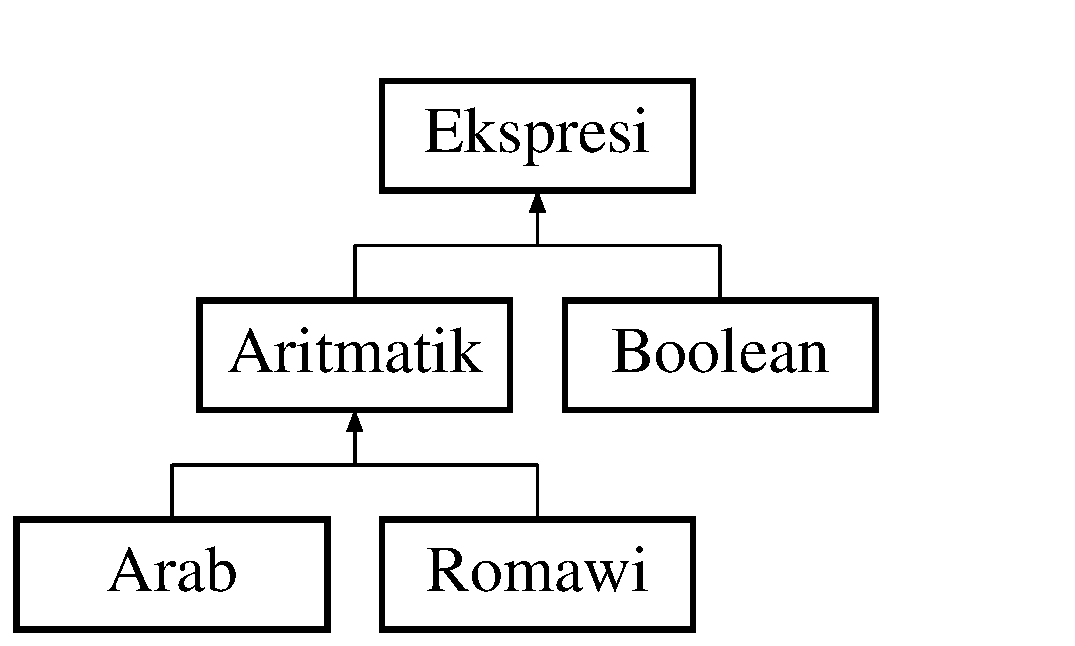
\includegraphics[height=3.000000cm]{class_ekspresi}
\end{center}
\end{figure}
\subsection*{Public Member Functions}
\begin{DoxyCompactItemize}
\item 
\hyperlink{class_ekspresi_af2e8f739d94a28af80105222107f4d3e}{Ekspresi} ()
\item 
\hyperlink{class_ekspresi_ac39dbe3ebc56004cfb24649c36cb29a5}{Ekspresi} (std\+::string, int)
\item 
\hyperlink{class_ekspresi_ac385e453495f162dc5d98ded7f1ea30a}{$\sim$\+Ekspresi} ()
\item 
std\+::string \hyperlink{class_ekspresi_a40f6b3556c45c99ba94d4f19a420c025}{get\+Ekspresi} ()
\item 
int \hyperlink{class_ekspresi_aa1a9b559652450e0759da6b8231a2dd4}{get\+Initial\+Id} ()
\item 
void \hyperlink{class_ekspresi_a554bbd85ea4c39188e9b40a79993d048}{set\+Ekspresi} (std\+::string)
\item 
virtual bool \hyperlink{class_ekspresi_ab742ee9ef7a7bc49ea9d3d96eae69e04}{is\+Operan} (std\+::string)=0
\item 
virtual bool \hyperlink{class_ekspresi_a224d9cae2ee4d104d7ece7b853746dfc}{is\+Operator} (std\+::string)=0
\item 
virtual bool \hyperlink{class_ekspresi_a52ccbd282ee50c4c3d58eab0d662f0f9}{higher\+Precedence} (std\+::string, std\+::string)=0
\end{DoxyCompactItemize}
\subsection*{Protected Member Functions}
\begin{DoxyCompactItemize}
\item 
virtual int \hyperlink{class_ekspresi_a1177f9babe3330a4f04adbac396e0e0e}{get\+Operator\+Weight} (std\+::string)=0
\item 
void \hyperlink{class_ekspresi_aeb458e4d9a607aac1aa021bc13fde362}{Prefix\+To\+Postfix} ()
\item 
void \hyperlink{class_ekspresi_acb880011d232d3624844eab3753e6dbd}{Infix\+To\+Postfix} ()
\end{DoxyCompactItemize}
\subsection*{Protected Attributes}
\begin{DoxyCompactItemize}
\item 
std\+::string \hyperlink{class_ekspresi_a9d5082854ad50d47e63eb1bf4e263a3a}{ekspresi}
\item 
const int \hyperlink{class_ekspresi_a7f5e4a40d4388ce071287e2f961c2ff1}{id}
\end{DoxyCompactItemize}


\subsection{Constructor \& Destructor Documentation}
\hypertarget{class_ekspresi_af2e8f739d94a28af80105222107f4d3e}{}\index{Ekspresi@{Ekspresi}!Ekspresi@{Ekspresi}}
\index{Ekspresi@{Ekspresi}!Ekspresi@{Ekspresi}}
\subsubsection[{Ekspresi}]{\setlength{\rightskip}{0pt plus 5cm}Ekspresi\+::\+Ekspresi (
\begin{DoxyParamCaption}
{}
\end{DoxyParamCaption}
)}\label{class_ekspresi_af2e8f739d94a28af80105222107f4d3e}
A constructor. ekpresi =\char`\"{}\char`\"{} Memnginisialisasi id = Setting\+::\+Postfix dengan ctor initilization list \hypertarget{class_ekspresi_ac39dbe3ebc56004cfb24649c36cb29a5}{}\index{Ekspresi@{Ekspresi}!Ekspresi@{Ekspresi}}
\index{Ekspresi@{Ekspresi}!Ekspresi@{Ekspresi}}
\subsubsection[{Ekspresi}]{\setlength{\rightskip}{0pt plus 5cm}Ekspresi\+::\+Ekspresi (
\begin{DoxyParamCaption}
\item[{std\+::string}]{eks, }
\item[{int}]{mode}
\end{DoxyParamCaption}
)}\label{class_ekspresi_ac39dbe3ebc56004cfb24649c36cb29a5}
A constructor. mengisi ekspresi menjadi eks Memnginisialisasi id = mode dengan ctor initilization list 
\begin{DoxyParams}{Parameters}
{\em mode} & sebagai int \\
\hline
{\em eks} & sebagai string \\
\hline
\end{DoxyParams}
\hypertarget{class_ekspresi_ac385e453495f162dc5d98ded7f1ea30a}{}\index{Ekspresi@{Ekspresi}!````~Ekspresi@{$\sim$\+Ekspresi}}
\index{````~Ekspresi@{$\sim$\+Ekspresi}!Ekspresi@{Ekspresi}}
\subsubsection[{$\sim$\+Ekspresi}]{\setlength{\rightskip}{0pt plus 5cm}Ekspresi\+::$\sim$\+Ekspresi (
\begin{DoxyParamCaption}
{}
\end{DoxyParamCaption}
)}\label{class_ekspresi_ac385e453495f162dc5d98ded7f1ea30a}
A destructor. 

\subsection{Member Function Documentation}
\hypertarget{class_ekspresi_a40f6b3556c45c99ba94d4f19a420c025}{}\index{Ekspresi@{Ekspresi}!get\+Ekspresi@{get\+Ekspresi}}
\index{get\+Ekspresi@{get\+Ekspresi}!Ekspresi@{Ekspresi}}
\subsubsection[{get\+Ekspresi}]{\setlength{\rightskip}{0pt plus 5cm}std\+::string Ekspresi\+::get\+Ekspresi (
\begin{DoxyParamCaption}
{}
\end{DoxyParamCaption}
)}\label{class_ekspresi_a40f6b3556c45c99ba94d4f19a420c025}
A getter. mendapatkan ekspresi \begin{DoxyReturn}{Returns}
string sebagai ekspresi 
\end{DoxyReturn}
\hypertarget{class_ekspresi_aa1a9b559652450e0759da6b8231a2dd4}{}\index{Ekspresi@{Ekspresi}!get\+Initial\+Id@{get\+Initial\+Id}}
\index{get\+Initial\+Id@{get\+Initial\+Id}!Ekspresi@{Ekspresi}}
\subsubsection[{get\+Initial\+Id}]{\setlength{\rightskip}{0pt plus 5cm}int Ekspresi\+::get\+Initial\+Id (
\begin{DoxyParamCaption}
{}
\end{DoxyParamCaption}
)}\label{class_ekspresi_aa1a9b559652450e0759da6b8231a2dd4}
A getter. mendapatkan id \begin{DoxyReturn}{Returns}
id , integer 
\end{DoxyReturn}
\hypertarget{class_ekspresi_a1177f9babe3330a4f04adbac396e0e0e}{}\index{Ekspresi@{Ekspresi}!get\+Operator\+Weight@{get\+Operator\+Weight}}
\index{get\+Operator\+Weight@{get\+Operator\+Weight}!Ekspresi@{Ekspresi}}
\subsubsection[{get\+Operator\+Weight}]{\setlength{\rightskip}{0pt plus 5cm}virtual int Ekspresi\+::get\+Operator\+Weight (
\begin{DoxyParamCaption}
\item[{std\+::string}]{}
\end{DoxyParamCaption}
)\hspace{0.3cm}{\ttfamily [protected]}, {\ttfamily [pure virtual]}}\label{class_ekspresi_a1177f9babe3330a4f04adbac396e0e0e}
a protected pure virtual member 
\begin{DoxyParams}{Parameters}
{\em oprt} & yang berupa string \\
\hline
\end{DoxyParams}
\begin{DoxyReturn}{Returns}
integer yang berupa bobot 
\end{DoxyReturn}


Implemented in \hyperlink{class_aritmatik_acb650d44adc6254fb3e0f027838af2db}{Aritmatik}.

\hypertarget{class_ekspresi_a52ccbd282ee50c4c3d58eab0d662f0f9}{}\index{Ekspresi@{Ekspresi}!higher\+Precedence@{higher\+Precedence}}
\index{higher\+Precedence@{higher\+Precedence}!Ekspresi@{Ekspresi}}
\subsubsection[{higher\+Precedence}]{\setlength{\rightskip}{0pt plus 5cm}virtual bool Ekspresi\+::higher\+Precedence (
\begin{DoxyParamCaption}
\item[{std\+::string}]{, }
\item[{std\+::string}]{}
\end{DoxyParamCaption}
)\hspace{0.3cm}{\ttfamily [pure virtual]}}\label{class_ekspresi_a52ccbd282ee50c4c3d58eab0d662f0f9}
A pure virtual member. 
\begin{DoxyParams}{Parameters}
{\em high} & yang berupa string \\
\hline
{\em low} & yang berupa string \\
\hline
\end{DoxyParams}
\begin{DoxyReturn}{Returns}
bool yang berupa true jika bobot high $>$ bobot low 
\end{DoxyReturn}


Implemented in \hyperlink{class_aritmatik_a2bdb89adcf3b187382a40f3c66e8b649}{Aritmatik}, and \hyperlink{class_boolean_a98d763cbf5a4593f5ec268bf7ccd3553}{Boolean}.

\hypertarget{class_ekspresi_acb880011d232d3624844eab3753e6dbd}{}\index{Ekspresi@{Ekspresi}!Infix\+To\+Postfix@{Infix\+To\+Postfix}}
\index{Infix\+To\+Postfix@{Infix\+To\+Postfix}!Ekspresi@{Ekspresi}}
\subsubsection[{Infix\+To\+Postfix}]{\setlength{\rightskip}{0pt plus 5cm}void Ekspresi\+::\+Infix\+To\+Postfix (
\begin{DoxyParamCaption}
{}
\end{DoxyParamCaption}
)\hspace{0.3cm}{\ttfamily [protected]}}\label{class_ekspresi_acb880011d232d3624844eab3753e6dbd}
protected method mengubah dari infix menjadi postfix \hypertarget{class_ekspresi_ab742ee9ef7a7bc49ea9d3d96eae69e04}{}\index{Ekspresi@{Ekspresi}!is\+Operan@{is\+Operan}}
\index{is\+Operan@{is\+Operan}!Ekspresi@{Ekspresi}}
\subsubsection[{is\+Operan}]{\setlength{\rightskip}{0pt plus 5cm}virtual bool Ekspresi\+::is\+Operan (
\begin{DoxyParamCaption}
\item[{std\+::string}]{}
\end{DoxyParamCaption}
)\hspace{0.3cm}{\ttfamily [pure virtual]}}\label{class_ekspresi_ab742ee9ef7a7bc49ea9d3d96eae69e04}
A pure virtual member. 
\begin{DoxyParams}{Parameters}
{\em string} & \\
\hline
\end{DoxyParams}
\begin{DoxyReturn}{Returns}
bool yang berupa true jika string adalah operan 
\end{DoxyReturn}


Implemented in \hyperlink{class_aritmatik_ad3bebd263fb4d94e850848c282f80d6b}{Aritmatik}, and \hyperlink{class_boolean_a9c5afca5ecb28f04ac727a56d646d057}{Boolean}.

\hypertarget{class_ekspresi_a224d9cae2ee4d104d7ece7b853746dfc}{}\index{Ekspresi@{Ekspresi}!is\+Operator@{is\+Operator}}
\index{is\+Operator@{is\+Operator}!Ekspresi@{Ekspresi}}
\subsubsection[{is\+Operator}]{\setlength{\rightskip}{0pt plus 5cm}virtual bool Ekspresi\+::is\+Operator (
\begin{DoxyParamCaption}
\item[{std\+::string}]{}
\end{DoxyParamCaption}
)\hspace{0.3cm}{\ttfamily [pure virtual]}}\label{class_ekspresi_a224d9cae2ee4d104d7ece7b853746dfc}
A pure virtual member. 
\begin{DoxyParams}{Parameters}
{\em string} & \\
\hline
\end{DoxyParams}
\begin{DoxyReturn}{Returns}
bool yang berupa true jika string adalah operator 
\end{DoxyReturn}


Implemented in \hyperlink{class_aritmatik_a22df02b3a845fd0af3e1bae28121ba99}{Aritmatik}, and \hyperlink{class_boolean_a37e98802c20820e8cdbbfa38232b4930}{Boolean}.

\hypertarget{class_ekspresi_aeb458e4d9a607aac1aa021bc13fde362}{}\index{Ekspresi@{Ekspresi}!Prefix\+To\+Postfix@{Prefix\+To\+Postfix}}
\index{Prefix\+To\+Postfix@{Prefix\+To\+Postfix}!Ekspresi@{Ekspresi}}
\subsubsection[{Prefix\+To\+Postfix}]{\setlength{\rightskip}{0pt plus 5cm}void Ekspresi\+::\+Prefix\+To\+Postfix (
\begin{DoxyParamCaption}
{}
\end{DoxyParamCaption}
)\hspace{0.3cm}{\ttfamily [protected]}}\label{class_ekspresi_aeb458e4d9a607aac1aa021bc13fde362}
protected method mengubah dari prefix menjadi postfix \hypertarget{class_ekspresi_a554bbd85ea4c39188e9b40a79993d048}{}\index{Ekspresi@{Ekspresi}!set\+Ekspresi@{set\+Ekspresi}}
\index{set\+Ekspresi@{set\+Ekspresi}!Ekspresi@{Ekspresi}}
\subsubsection[{set\+Ekspresi}]{\setlength{\rightskip}{0pt plus 5cm}void Ekspresi\+::set\+Ekspresi (
\begin{DoxyParamCaption}
\item[{std\+::string}]{eks}
\end{DoxyParamCaption}
)}\label{class_ekspresi_a554bbd85ea4c39188e9b40a79993d048}
A setter. menset string dengan eks 
\begin{DoxyParams}{Parameters}
{\em eks} & \\
\hline
\end{DoxyParams}


\subsection{Member Data Documentation}
\hypertarget{class_ekspresi_a9d5082854ad50d47e63eb1bf4e263a3a}{}\index{Ekspresi@{Ekspresi}!ekspresi@{ekspresi}}
\index{ekspresi@{ekspresi}!Ekspresi@{Ekspresi}}
\subsubsection[{ekspresi}]{\setlength{\rightskip}{0pt plus 5cm}std\+::string Ekspresi\+::ekspresi\hspace{0.3cm}{\ttfamily [protected]}}\label{class_ekspresi_a9d5082854ad50d47e63eb1bf4e263a3a}
protected variable yang berupa string \hypertarget{class_ekspresi_a7f5e4a40d4388ce071287e2f961c2ff1}{}\index{Ekspresi@{Ekspresi}!id@{id}}
\index{id@{id}!Ekspresi@{Ekspresi}}
\subsubsection[{id}]{\setlength{\rightskip}{0pt plus 5cm}const int Ekspresi\+::id\hspace{0.3cm}{\ttfamily [protected]}}\label{class_ekspresi_a7f5e4a40d4388ce071287e2f961c2ff1}
protected variable yang berupa konstanta integer 

The documentation for this class was generated from the following files\+:\begin{DoxyCompactItemize}
\item 
Ekspresi.\+h\item 
Ekspresi.\+cpp\end{DoxyCompactItemize}

\hypertarget{class_romawi}{}\section{Romawi Class Reference}
\label{class_romawi}\index{Romawi@{Romawi}}
Inheritance diagram for Romawi\+:\begin{figure}[H]
\begin{center}
\leavevmode
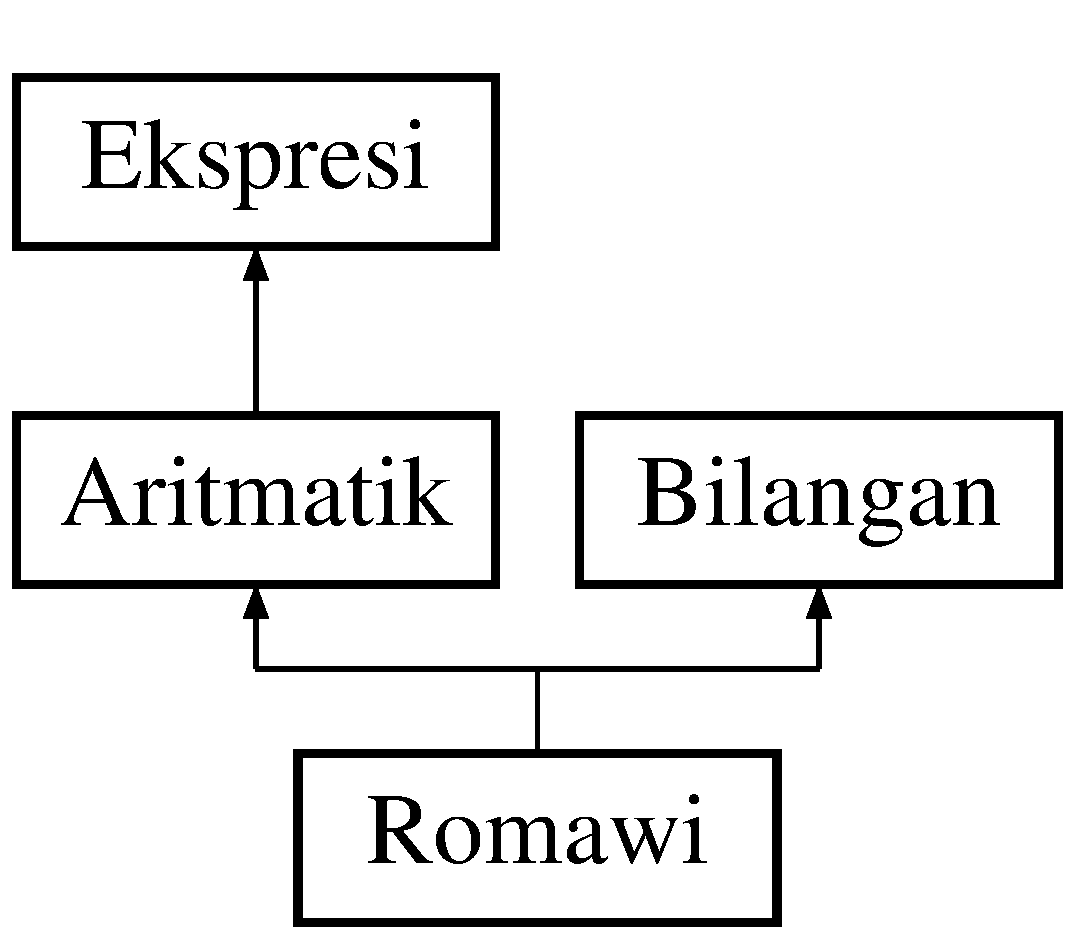
\includegraphics[height=3.000000cm]{class_romawi}
\end{center}
\end{figure}
\subsection*{Public Member Functions}
\begin{DoxyCompactItemize}
\item 
\hyperlink{class_romawi_ae904ce8e098ff7eb906ec3996ba877f5}{Romawi} ()
\item 
\hyperlink{class_romawi_a49007cbd3862aef2a71fb5a6c8f0a67a}{Romawi} (std\+::string, int)
\item 
\hyperlink{class_romawi_a208bcc4479304450d7b0f578534f18db}{$\sim$\+Romawi} ()
\item 
int \hyperlink{class_romawi_a6fabccebadf8807fbdd50a0c45b093e2}{calculate} ()
\item 
int \hyperlink{class_romawi_aaa81d7f110f3baabad7571fec567bb12}{binary\+Opt} (std\+::string, int, int)
\item 
int \hyperlink{class_romawi_af98f44a64aa48746641faac4dac3fb33}{unary\+Opt} (std\+::string, int)
\item 
int \hyperlink{class_romawi_ae884d8a5a65c397fe53a05af8f0747f4}{to\+Int} (std\+::string)
\item 
std\+::string \hyperlink{class_romawi_a338773fe7e1762d5c52e803ba2957205}{to\+String} (int)
\end{DoxyCompactItemize}
\subsection*{Additional Inherited Members}


\subsection{Constructor \& Destructor Documentation}
\hypertarget{class_romawi_ae904ce8e098ff7eb906ec3996ba877f5}{}\index{Romawi@{Romawi}!Romawi@{Romawi}}
\index{Romawi@{Romawi}!Romawi@{Romawi}}
\subsubsection[{Romawi}]{\setlength{\rightskip}{0pt plus 5cm}Romawi\+::\+Romawi (
\begin{DoxyParamCaption}
{}
\end{DoxyParamCaption}
)}\label{class_romawi_ae904ce8e098ff7eb906ec3996ba877f5}
A constructor. Membuat Objek \hyperlink{class_aritmatik}{Aritmatik} \hypertarget{class_romawi_a49007cbd3862aef2a71fb5a6c8f0a67a}{}\index{Romawi@{Romawi}!Romawi@{Romawi}}
\index{Romawi@{Romawi}!Romawi@{Romawi}}
\subsubsection[{Romawi}]{\setlength{\rightskip}{0pt plus 5cm}Romawi\+::\+Romawi (
\begin{DoxyParamCaption}
\item[{std\+::string}]{eks, }
\item[{int}]{\+\_\+mode}
\end{DoxyParamCaption}
)}\label{class_romawi_a49007cbd3862aef2a71fb5a6c8f0a67a}
A constructor. Membuat Objek \hyperlink{class_aritmatik}{Aritmatik} 
\begin{DoxyParams}{Parameters}
{\em eks} & sebuah string \\
\hline
{\em mode} & a yang berupa integer \\
\hline
\end{DoxyParams}
\hypertarget{class_romawi_a208bcc4479304450d7b0f578534f18db}{}\index{Romawi@{Romawi}!````~Romawi@{$\sim$\+Romawi}}
\index{````~Romawi@{$\sim$\+Romawi}!Romawi@{Romawi}}
\subsubsection[{$\sim$\+Romawi}]{\setlength{\rightskip}{0pt plus 5cm}Romawi\+::$\sim$\+Romawi (
\begin{DoxyParamCaption}
{}
\end{DoxyParamCaption}
)}\label{class_romawi_a208bcc4479304450d7b0f578534f18db}
A destructor. 

\subsection{Member Function Documentation}
\hypertarget{class_romawi_aaa81d7f110f3baabad7571fec567bb12}{}\index{Romawi@{Romawi}!binary\+Opt@{binary\+Opt}}
\index{binary\+Opt@{binary\+Opt}!Romawi@{Romawi}}
\subsubsection[{binary\+Opt}]{\setlength{\rightskip}{0pt plus 5cm}int Romawi\+::binary\+Opt (
\begin{DoxyParamCaption}
\item[{std\+::string}]{oprt, }
\item[{int}]{a, }
\item[{int}]{b}
\end{DoxyParamCaption}
)\hspace{0.3cm}{\ttfamily [virtual]}}\label{class_romawi_aaa81d7f110f3baabad7571fec567bb12}
Method yang mengembalikan hasil dari operasi binary Menghitung dua buah integer 
\begin{DoxyParams}{Parameters}
{\em a} & sebuah integer \\
\hline
{\em b} & sebuah integer \\
\hline
\end{DoxyParams}
\begin{DoxyReturn}{Returns}
hasil perhitungan binary 
\end{DoxyReturn}


Implements \hyperlink{class_bilangan_acb958e0fade6bdfc3b6ce88bf57560bc}{Bilangan}.

\hypertarget{class_romawi_a6fabccebadf8807fbdd50a0c45b093e2}{}\index{Romawi@{Romawi}!calculate@{calculate}}
\index{calculate@{calculate}!Romawi@{Romawi}}
\subsubsection[{calculate}]{\setlength{\rightskip}{0pt plus 5cm}int Romawi\+::calculate (
\begin{DoxyParamCaption}
{}
\end{DoxyParamCaption}
)\hspace{0.3cm}{\ttfamily [virtual]}}\label{class_romawi_a6fabccebadf8807fbdd50a0c45b093e2}
Method yang mengembalikan hasil perhitungan Menghitung string postfix dengan stack. \begin{DoxySeeAlso}{See also}
\hyperlink{class_romawi_aaa81d7f110f3baabad7571fec567bb12}{binary\+Opt} 

\hyperlink{class_romawi_af98f44a64aa48746641faac4dac3fb33}{unary\+Opt} 

\hyperlink{class_romawi_ae884d8a5a65c397fe53a05af8f0747f4}{to\+Int} 
\end{DoxySeeAlso}
\begin{DoxyReturn}{Returns}
hasil perhitungan 
\end{DoxyReturn}


Implements \hyperlink{class_bilangan_a519c33685bdc47e8386037ac8d2bfaa6}{Bilangan}.

\hypertarget{class_romawi_ae884d8a5a65c397fe53a05af8f0747f4}{}\index{Romawi@{Romawi}!to\+Int@{to\+Int}}
\index{to\+Int@{to\+Int}!Romawi@{Romawi}}
\subsubsection[{to\+Int}]{\setlength{\rightskip}{0pt plus 5cm}int Romawi\+::to\+Int (
\begin{DoxyParamCaption}
\item[{std\+::string}]{str}
\end{DoxyParamCaption}
)\hspace{0.3cm}{\ttfamily [virtual]}}\label{class_romawi_ae884d8a5a65c397fe53a05af8f0747f4}
Method yang mengembalikan integet Mengubah string menjadi Integer 
\begin{DoxyParams}{Parameters}
{\em str} & sebuah string \\
\hline
\end{DoxyParams}
\begin{DoxyReturn}{Returns}
bilangan integer hasil convert 
\end{DoxyReturn}


Implements \hyperlink{class_bilangan_ab4fd66bd8e9179176f97f8b856eda103}{Bilangan}.

\hypertarget{class_romawi_a338773fe7e1762d5c52e803ba2957205}{}\index{Romawi@{Romawi}!to\+String@{to\+String}}
\index{to\+String@{to\+String}!Romawi@{Romawi}}
\subsubsection[{to\+String}]{\setlength{\rightskip}{0pt plus 5cm}std\+::string Romawi\+::to\+String (
\begin{DoxyParamCaption}
\item[{int}]{bil}
\end{DoxyParamCaption}
)\hspace{0.3cm}{\ttfamily [virtual]}}\label{class_romawi_a338773fe7e1762d5c52e803ba2957205}
Method yang mengembalikan string Mengubah Integer menjadi string 
\begin{DoxyParams}{Parameters}
{\em bil} & sebuah integer \\
\hline
\end{DoxyParams}
\begin{DoxyReturn}{Returns}
the string 
\end{DoxyReturn}


Implements \hyperlink{class_bilangan_ac712d0d2b78dabad769b0b1e9cef8dc6}{Bilangan}.

\hypertarget{class_romawi_af98f44a64aa48746641faac4dac3fb33}{}\index{Romawi@{Romawi}!unary\+Opt@{unary\+Opt}}
\index{unary\+Opt@{unary\+Opt}!Romawi@{Romawi}}
\subsubsection[{unary\+Opt}]{\setlength{\rightskip}{0pt plus 5cm}int Romawi\+::unary\+Opt (
\begin{DoxyParamCaption}
\item[{std\+::string}]{oprt, }
\item[{int}]{a}
\end{DoxyParamCaption}
)\hspace{0.3cm}{\ttfamily [virtual]}}\label{class_romawi_af98f44a64aa48746641faac4dac3fb33}
Method yang mengembalikan hasil dari operasi unary Menghitung satu buah integer 
\begin{DoxyParams}{Parameters}
{\em a} & sebuah integer \\
\hline
\end{DoxyParams}
\begin{DoxyReturn}{Returns}
bilangan integer sebuah hasil 
\end{DoxyReturn}


Implements \hyperlink{class_bilangan_af812d372ad4de1afe2e6a4dc9e8f95ef}{Bilangan}.



The documentation for this class was generated from the following files\+:\begin{DoxyCompactItemize}
\item 
Romawi.\+h\item 
Romawi.\+cpp\end{DoxyCompactItemize}

\hypertarget{class_romawi_exp}{}\section{Romawi\+Exp Class Reference}
\label{class_romawi_exp}\index{Romawi\+Exp@{Romawi\+Exp}}
\subsection*{Public Member Functions}
\begin{DoxyCompactItemize}
\item 
\hyperlink{class_romawi_exp_aaea9845b6d3fc3c560f0c06d8e2db5ed}{Romawi\+Exp} (int)
\item 
\hyperlink{class_romawi_exp_a6782f940b6d964686c32bac480310619}{Romawi\+Exp} (const \hyperlink{class_romawi_exp}{Romawi\+Exp} \&)
\item 
void \hyperlink{class_romawi_exp_a299d3afa53df2d3445c8b75614723b9a}{display\+Msg} ()
\end{DoxyCompactItemize}


\subsection{Constructor \& Destructor Documentation}
\hypertarget{class_romawi_exp_aaea9845b6d3fc3c560f0c06d8e2db5ed}{}\index{Romawi\+Exp@{Romawi\+Exp}!Romawi\+Exp@{Romawi\+Exp}}
\index{Romawi\+Exp@{Romawi\+Exp}!Romawi\+Exp@{Romawi\+Exp}}
\subsubsection[{Romawi\+Exp}]{\setlength{\rightskip}{0pt plus 5cm}Romawi\+Exp\+::\+Romawi\+Exp (
\begin{DoxyParamCaption}
\item[{int}]{id}
\end{DoxyParamCaption}
)}\label{class_romawi_exp_aaea9845b6d3fc3c560f0c06d8e2db5ed}
A constructor. Memnginisialisasi msg\+\_\+id = id dengan ctor initilization list 
\begin{DoxyParams}{Parameters}
{\em id} & sebagai int \\
\hline
\end{DoxyParams}
\hypertarget{class_romawi_exp_a6782f940b6d964686c32bac480310619}{}\index{Romawi\+Exp@{Romawi\+Exp}!Romawi\+Exp@{Romawi\+Exp}}
\index{Romawi\+Exp@{Romawi\+Exp}!Romawi\+Exp@{Romawi\+Exp}}
\subsubsection[{Romawi\+Exp}]{\setlength{\rightskip}{0pt plus 5cm}Romawi\+Exp\+::\+Romawi\+Exp (
\begin{DoxyParamCaption}
\item[{const {\bf Romawi\+Exp} \&}]{exp}
\end{DoxyParamCaption}
)}\label{class_romawi_exp_a6782f940b6d964686c32bac480310619}
A copy constructor. Memnginisialisasi msg\+\_\+id = exp.\+msg\+\_\+id dengan ctor initilization list 
\begin{DoxyParams}{Parameters}
{\em exp} & sebagai konstanta reference dari Romawib\+Exp \\
\hline
\end{DoxyParams}


\subsection{Member Function Documentation}
\hypertarget{class_romawi_exp_a299d3afa53df2d3445c8b75614723b9a}{}\index{Romawi\+Exp@{Romawi\+Exp}!display\+Msg@{display\+Msg}}
\index{display\+Msg@{display\+Msg}!Romawi\+Exp@{Romawi\+Exp}}
\subsubsection[{display\+Msg}]{\setlength{\rightskip}{0pt plus 5cm}void Romawi\+Exp\+::display\+Msg (
\begin{DoxyParamCaption}
{}
\end{DoxyParamCaption}
)}\label{class_romawi_exp_a299d3afa53df2d3445c8b75614723b9a}
A void to display the string ( msg\mbox{[}\mbox{]}). Memngoutput msg\mbox{[}msg\+\_\+id\mbox{]} 

The documentation for this class was generated from the following files\+:\begin{DoxyCompactItemize}
\item 
Romawi\+Exp.\+h\item 
Romawi\+Exp.\+cpp\end{DoxyCompactItemize}

%--- End generated contents ---

% Index
\backmatter
\newpage
\phantomsection
\clearemptydoublepage
\addcontentsline{toc}{chapter}{Index}
\printindex

\end{document}
